% Capítulo 5 
\chapter{Evaluation}

This chapter addresses to check the suitability of the FISVER approach in provisioning cloud-enabled Smart Surveillance based transportation-safety systems. In general, the success of smart surveillance based transportation-safety system depends on deploying a software architecture with scalable, robust, and computationally efficient capabilities.

With the aim to obtain accurate insights, a real testbed that prototypes the FISVER framework is deployed. In evaluating the proposed framework, a set of experiments was conducted in two different scenarios taking into account a regular transportation-safety use-case for close to reality experimentation, as described in next session.

\section{Testbed Set of Experiments}

Considering that Smart Surveillance based transportation-safety system imposes higher requirements than those used in typical surveillance applications, computational resource consumption benchmarking in varying use case behavior is required during runtime. Following the guidelines of similar work available in the literature\cite{Evaluation1}\cite{Evaluation6}, two testbed set of experiments are adopted in the evaluation model, namely Typical Deployment and FISVER Built-in. The Typical Deployment set of experiment is depicted in Figure \ref{fig:tydep}. 

\begin{figure}[!htb]
	\centering
 	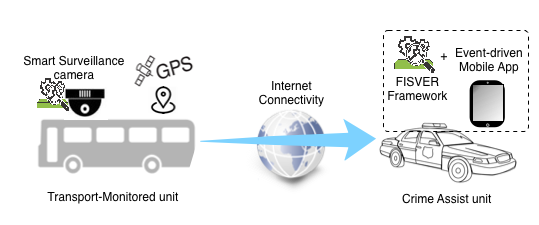
\includegraphics[scale=0.8]{Imagens/cap5_typical_testbed.png}
 	\caption{Typical Deployment testbed configuration}
 	\label{fig:tydep}
\end{figure}

On the one side, the Typical Deployment set of experiments aims to represent configuration sets regularly used in smart surveillance assessments for transportation-safety systems, following guidelines used in \cite{Typtest1}. For this dissertation, the configuration of the Typical Deployment set of experiments consider in-vehicle video surveillance subsystems sensing the cabin surroundings, and permanently streaming corresponding video flow towards a pre-assigned mobile application, leveraging available Internet connectivity. At the mobile application side, a video processing application using the Haar Cascade Features \cite{peng2011}, is in charge to process analytics on the received video streaming to detect objects and infer crime events. If any crime object matching is achieved, an alert event is dispatched to the notification area, so that reporting the user at the mobile device screen. The FISVER Built-in set of experiments is depicted in the Figure\ref{fig:fradep}.

\begin{figure}[!htb]'
	\centering
 	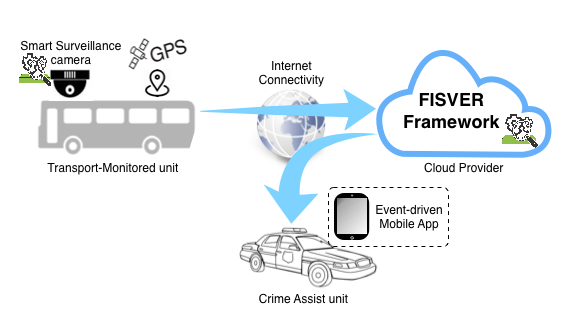
\includegraphics[scale=0.8]{Imagens/cap5_fisver_testbed.png}
 	\caption{FISVER Built-in testbed configuration}
 	\label{fig:fradep}
\end{figure}

On the other side, the FISVER Built-in set of experiments is in charge to prototyping the main subject of this dissertation. The configuration of the FISVER Built-in set of experiments is in compliance with the specifications detailed in the Chapter 4. In this set of experiments, the in-vehicle smart surveillance subsystem keeps constantly sensing the bus cabin surroundings, and uses the Haar Cascade Features to detect target crime objects locally. On detecting an object of potential security threat, the FISVER agent inside the camera composes a corresponding metadata set containing indication of the crime occurrence, GPS location of the vehicle and an image to sample the crime occurrence. Afterwards, it uses onboard Internet connectivity to send the metadata towards the cloud infrastructure featuring the FISVER approach. At the cloud, FISVER inspects the metadata to classify the indicated event. On confirming the crime event, it uses the derived GPS location to find in local data base the best crime assist. On the basis of finding the best crime assist unit, cloud FISVER in turn extends the corresponding metadata with the crime event classification, and sends it to the crime assist unit. 

To ensure that a similar processing deployment and comparative equality are maintained, the image processing algorithms are deployed in a Java\footnote[20]{Java. https://www.java.com/en/. Accessed on December 12th, 2015.} virtual machine that is called C++\footnote[21]{C++. http://www.cplusplus.com/. Accessed on December 12th, 2015.} native library. This was designed with aid of OpenCV\footnote[22]{OpenCV. http://opencv.org/. Accessed on December 12th, 2015.} , to create image manipulations and deploy the haar cascade feature algorithm. 

A Typical NDK\footnote[23]{NDK. http://developer.android.com/ndk/index.html. Accessed on December 12th, 2015.} Scenario is used to make native library loading for the Android mobile application. The native library loads are made through JNI for the FISVER Built-in set of experiments.

\section{Methodology applied for the Assessments}

Four tests are assigned for each one of the set of experiments, with the perspective to allow examining the impact in the testbed behavior under different conditions imposed by varying rates of notification load that is offered to the system \cite{Evaluation2}. Before conducting the target experiments, the testbed was stressed with an amount of crime detect notifications from smart surveillance camera. The goal is to figure out the maximum capacity of the system in handling security notifications without crashing it \cite{Evaluation4}, for use as benchmarking reference. The stressing test reveals a load of 3,600 offered security notification, which were sent out during the period of one hour of the experimental time.

In order to ease the prototype experimentation, the in-vehicle smart surveillance based transportation-safety system is represented by a software application that generates a number of notifications over the course of their experimental time (i.e., one hour) following the poison distribution, similarly as in \cite{Evaluation3}. Four datasets are deployed, each with a variation in the number of security notifications in function of the total security notifications set (i.e.,  3,600), allowing following workloads: 30\% (1,080 notifications), 60\% (2,160 notifications), 90\% (3,240 notification) and 120\% (4,320 notification). 

\section{Result Analysis}

On the basis that cloud-enabled smart surveillance based transportation-safety systems have critical performance issues, it is fundamental to adopt accurate benchmarking for obtaining consistent insights in multiple dimensions of resource consumption and optimization rates\cite{Evaluation5}. For the benchmarking model, the decision is to concentrate in the mobile device performance parameters, which is justified by the need on  obtaining insights in the perspective of the most agility demanding subsystem in the framework, the crime assist unit which will deal on the crime at the end.  

Assessments in the performance aspects at both in-vehicle and cloud FISVER subsystems are interesting and relevant, at the end the performance in the mobile unit brings the concrete view in overall interworking operations and user experience. Average rates in CPU utilization load, download/upload throughput and battery consumption on the event-driven mobile application side for the two set of experiments, are used as key performance information. To understand the behavior characteristics resulting from the surveillance system’s configurations, the benchmarking considers analysis in the runtime statistics collected while running the applications on the four workloads corresponding to each set of experiments. Each experiment is repeated 10 times, whereby averaging results are plotted to produce graphs, considering a confidence interval of 95\%.

\subsection{CPU Load Analytics}
\label{CPUAnalytics}

In regards to cloud-enabled Smart Surveillance systems, the list of major concerns facing these systems include scalability, ubiquitous access to sensory data, event processing overhead, and massive storage requirements \cite{Anwar_Hossain}. All of them together demand optimized service approach, and thus CPU utilization load is an important measure to estimate effectiveness on system performance. The CPU load analytics envisages to studying the utilization rate that both FISVER Built-in and Typical Deployment features take to the mobile device in the testbed with the varying offered notification load. The results of the CPU load obtained in both experiments are shown in Figure \ref{fig:result2}.

\begin{figure}[htb]
	\centering
 	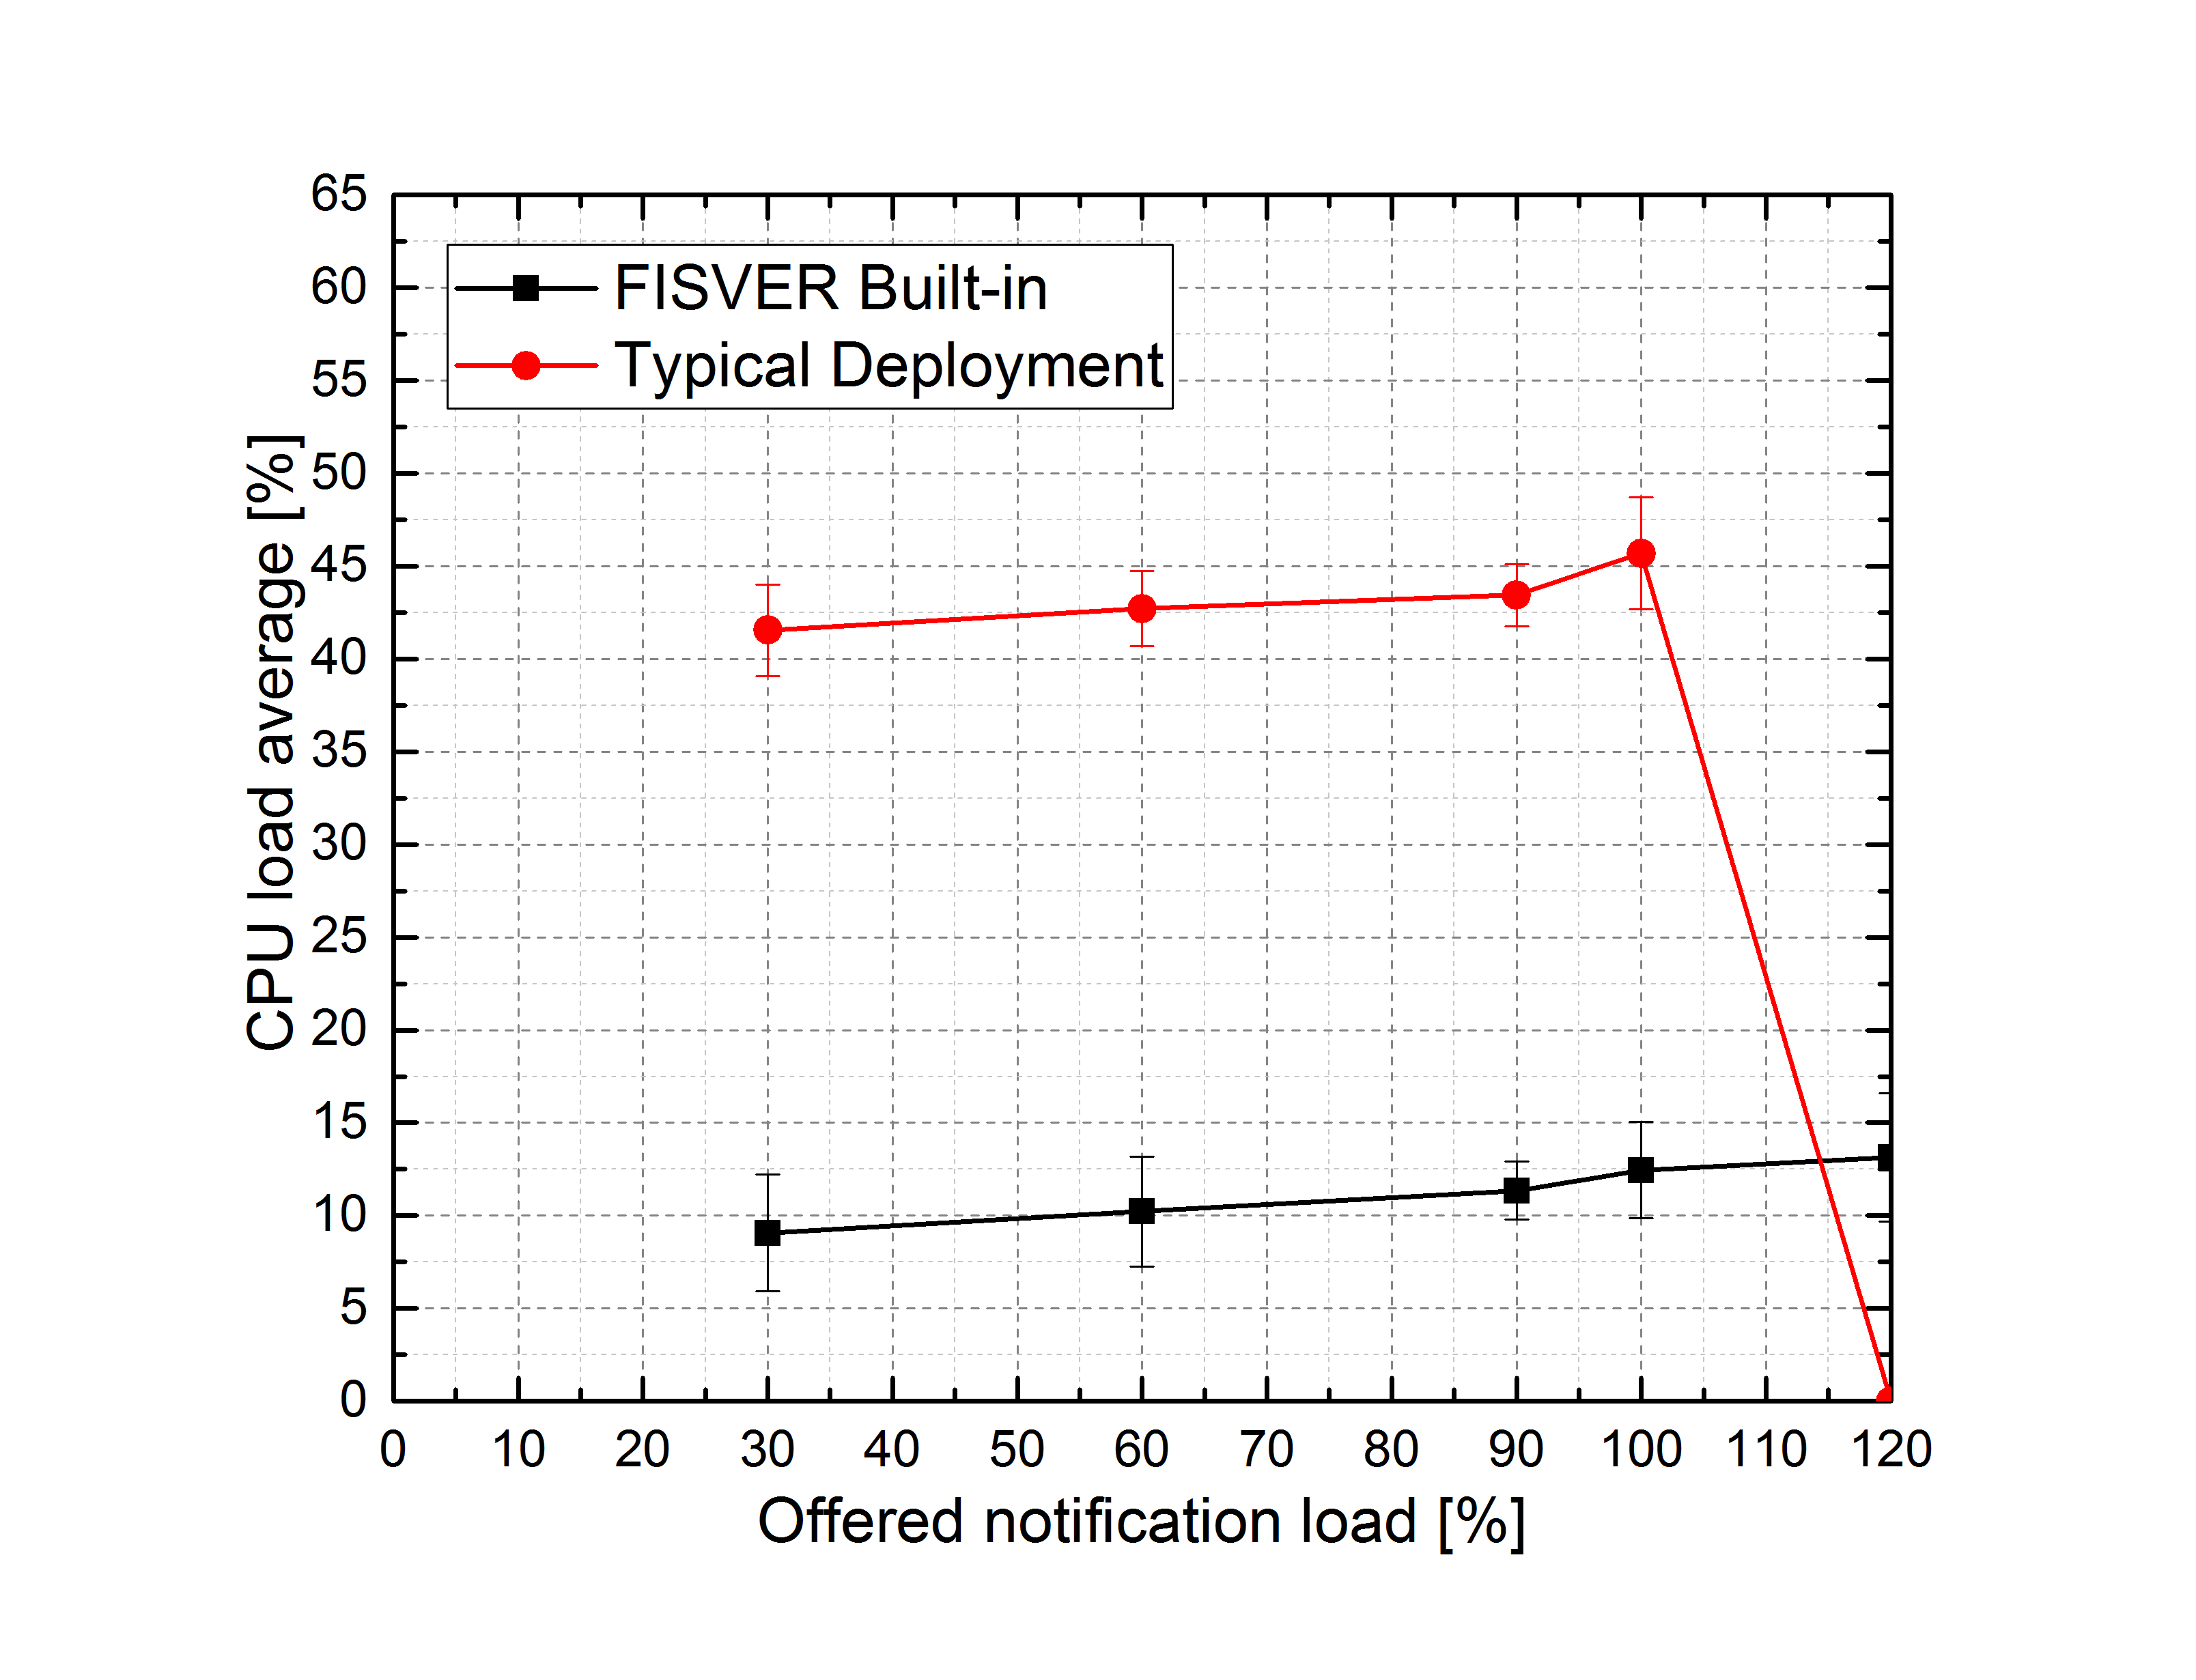
\includegraphics[scale=0.60]{Imagens/cap5_cpu.png}
 	\caption{CPU average load.}
 	\label{fig:result2}
\end{figure}

The results scratched in Figure \ref{fig:result2} confirm that the number of instances significantly affects the CPU consumption, which increases exponentially with the offered notification load scale. This behavior can be explained by the need to report the event-driven mobile application whenever the cloud service classifies a potential crime threat. Thus, the more target notifications are produced, the more crime event reports are generated and sent to the event-driven mobile application. The averaging CPU consumption in the FISVER Built-in set of experiments is of 10.94\%, whereas 44.84\% in the Typical Deployment testbed configuration. Thus, the results reveal that FISVER allows improving the CPU performance around 75.6\%.

The main reason for this improvement is obtained through the FISVER assistance, whereby all the Smart Surveillance complex tasks are carried out by both in-vehicle and cloud interworking subsystems, leaving the event-driven mobile application mostly in charge only to present the notification to the user. It is important to highlight that the Typical Deployment is unable to achieve the end of the experiments when submitted to 120\% of the offered notification load, because the system freezes by processing overload.

\subsection{Network Bandwidth Analytics}
\label{NetAnalytics}

The analysis in networking behavior has as main objective to observe the impact that the FISVER proposal takes in transport resources from the underlying intercommunication system. This set of analysis play a key role in estimating the system scalability, since networking imposes challenges and issues with regard to QoE, responsiveness, cost and survivability, specially in resource constrained mobile devices. For that, bandwidth consumption rates during both downstream (i.e., infrastructure/in-vehicle system to mobile app) and upstream (i.e., mobile app to infrastructure/in-vehicle system) service transport utilization are collected as measures for performance analysis across the different offered notification load. Figure (\ref{fig:result3}) illustrates the results in upload networking bandwidth utilization. 

\begin{figure}[htb]
	\centering
 	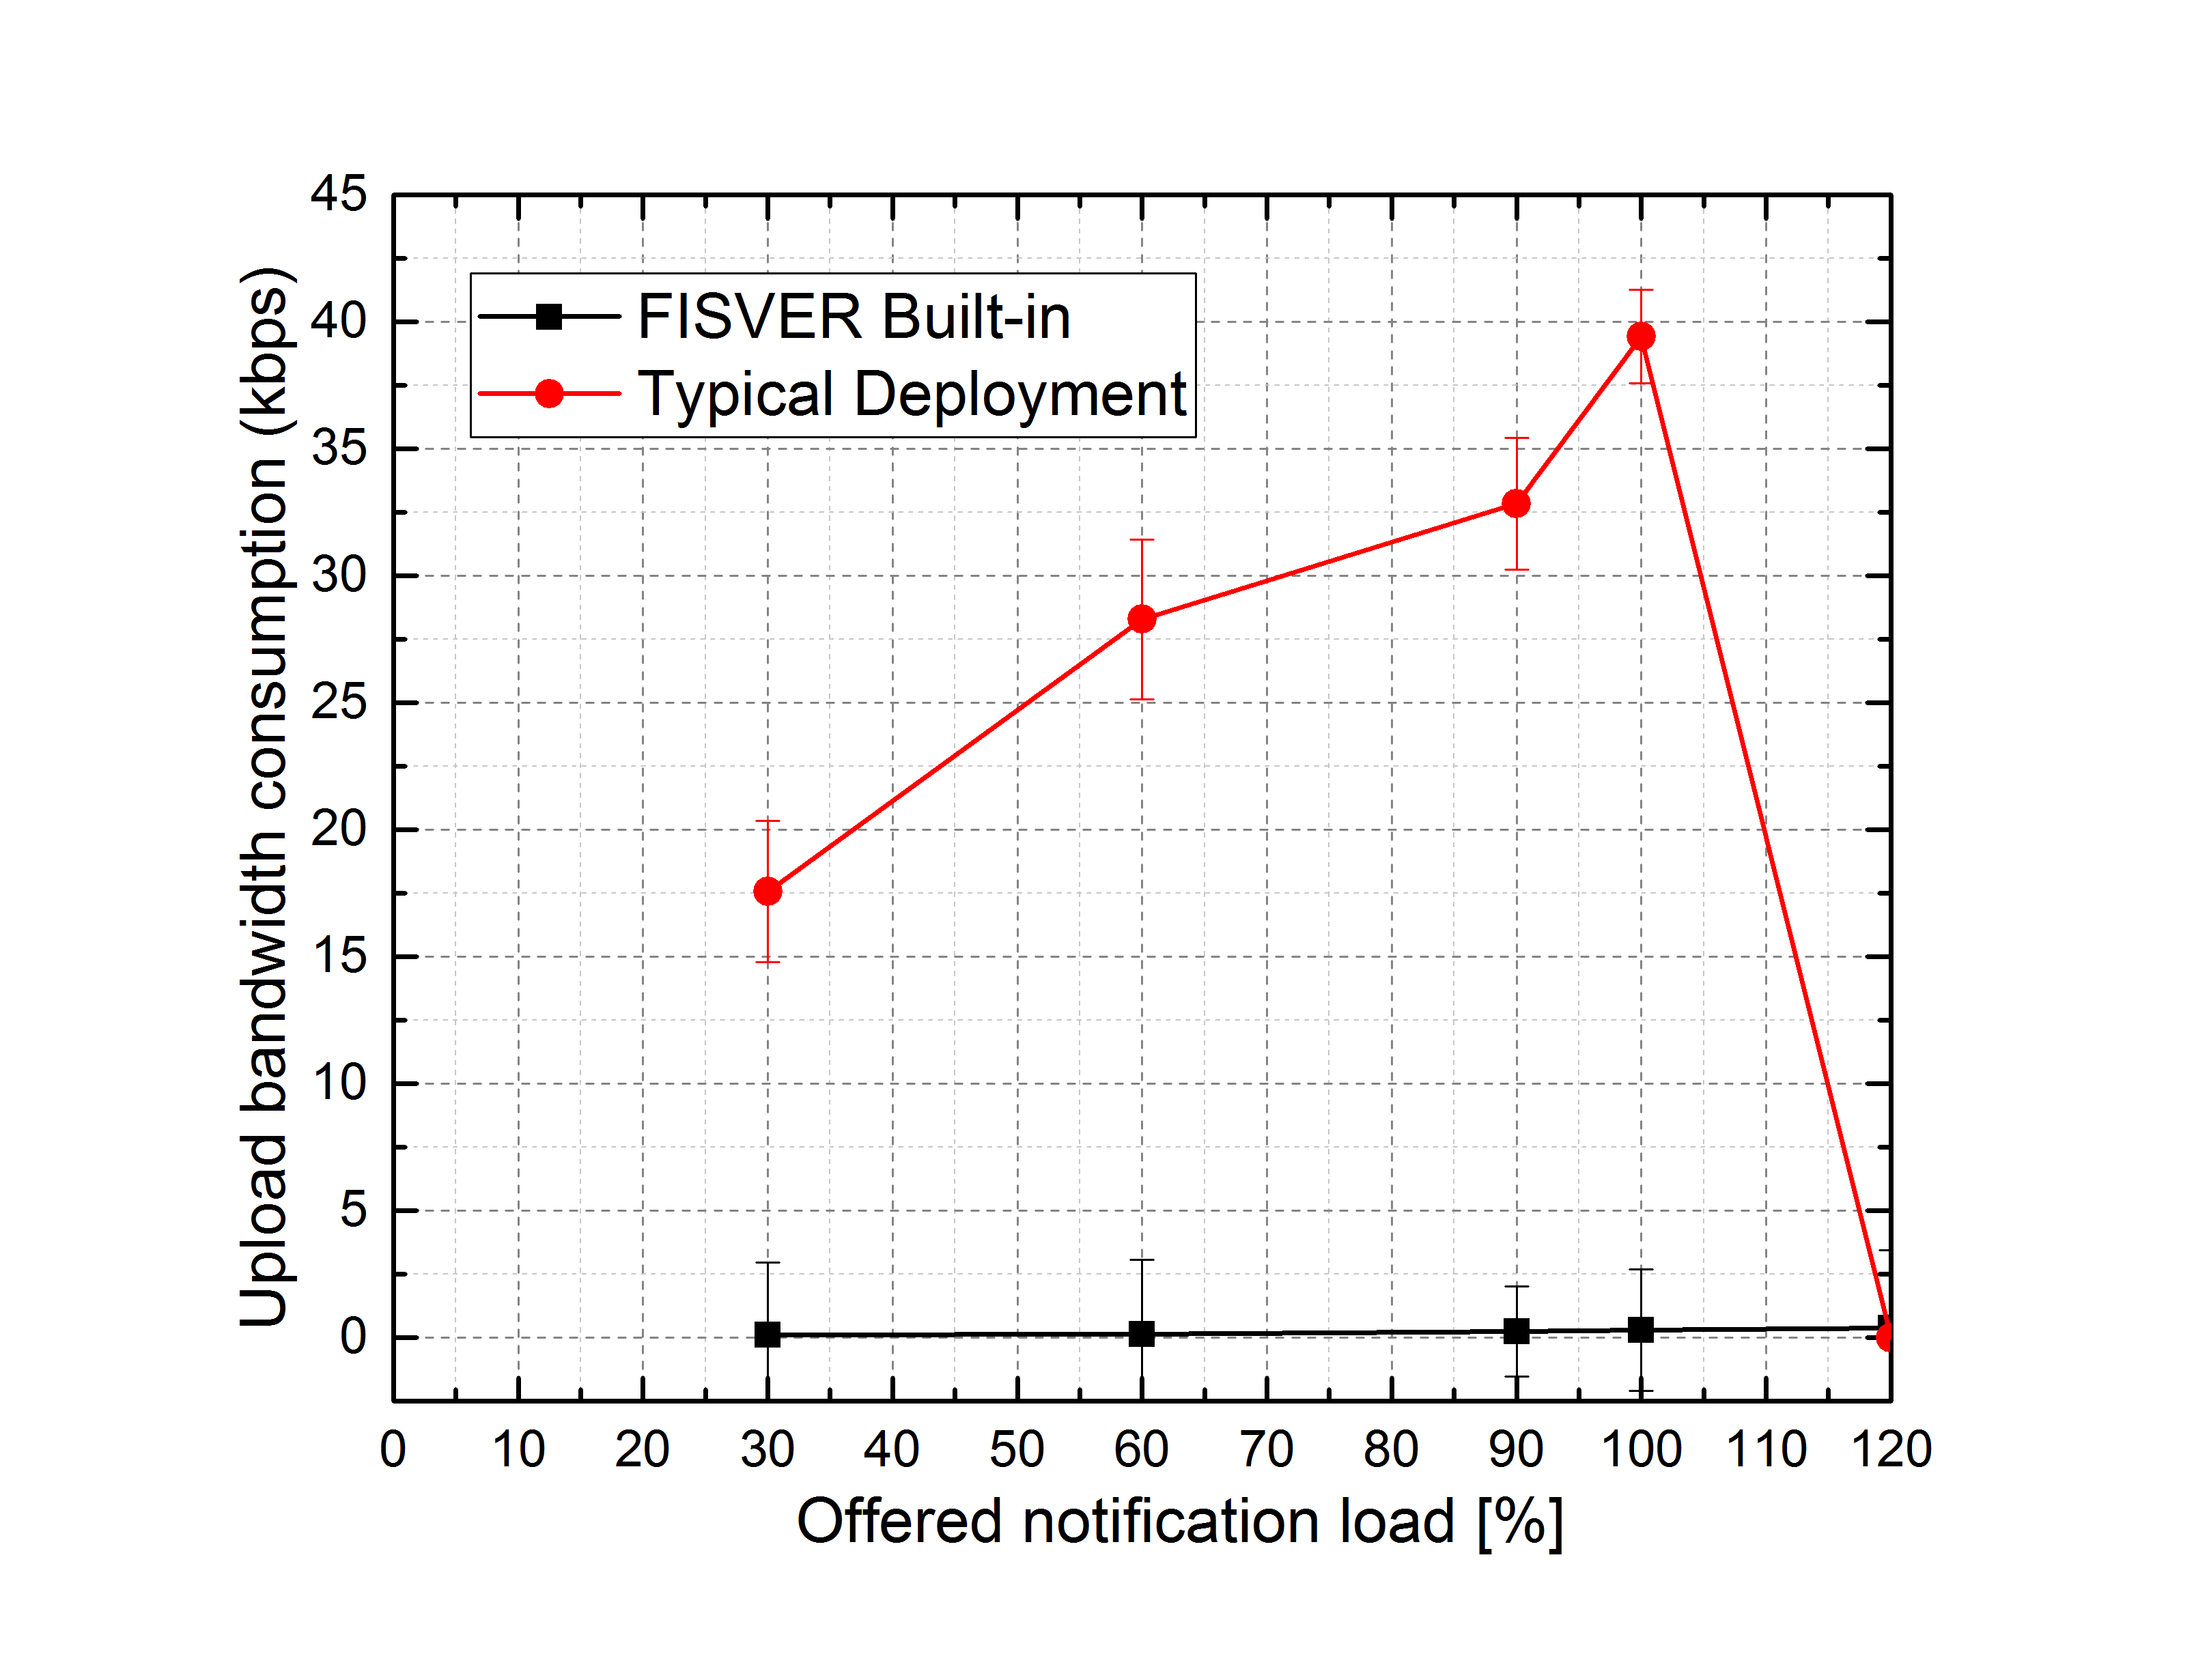
\includegraphics[scale=0.60]{Imagens/cap5_upload.png}
 	\caption{Upload bandwidth consumption.}
 	\label{fig:result3}
\end{figure}

As it can be observed in the Figure \ref{fig:result3}, the FISVER approach allows allocating around 0.2 kbps (i.s., less than 0.0018\% of the overall available bandwidth capacity) at the upstream service transport in the course of the experiments. On another hand, the Typical Deployment testbed configuration allocates an average of 29.53 kbps (26\%), therefore demonstrating an outstanding networking performance improvement of 99.993\%. This is achieved by concentrating all heavyweight processing task at the infrastructure, thus leaving the smartphone lightweight because the in-vehicle processing algorithm only dispatches crime events detections upon obtaining a positive target matching. Figure \ref{fig:result4} shows the average networking behavior in the downstream transport service during FISVER Built-in and Typical Deployment set of experiments.

\begin{figure}[htb]
	\centering
 	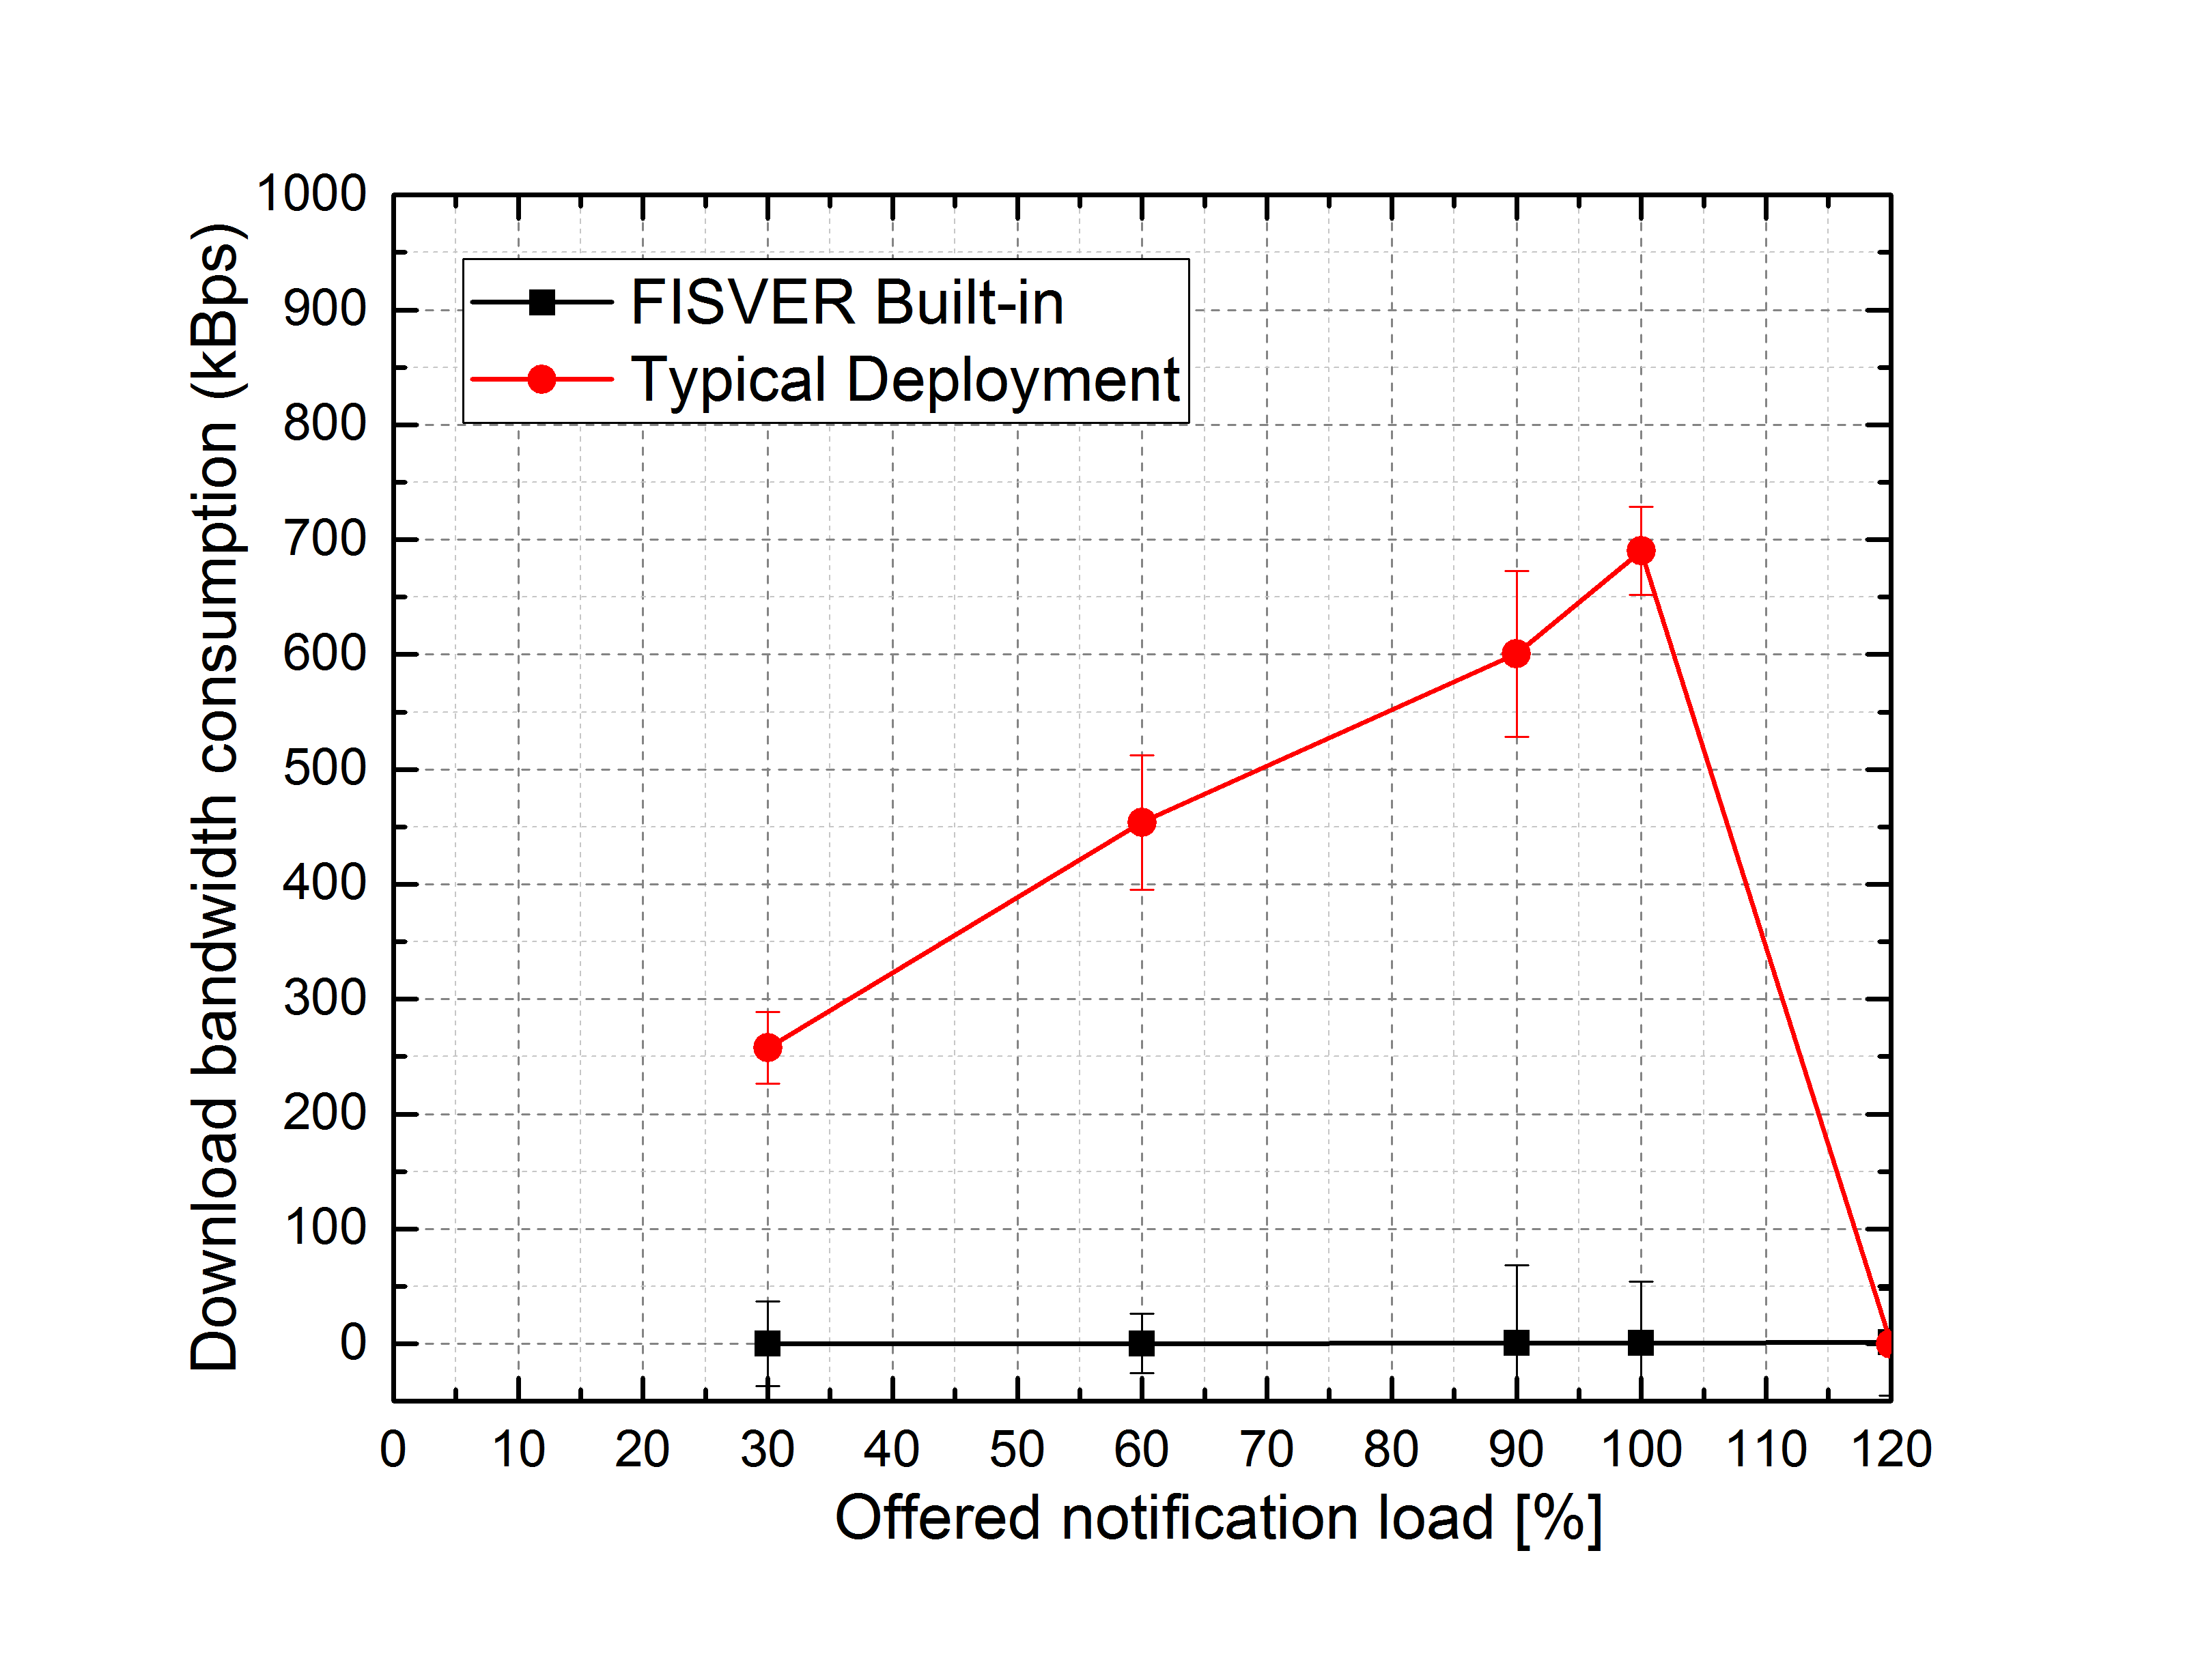
\includegraphics[scale=0.60]{Imagens/cap5_download.png}
 	\caption{Download bandwidth consumption.}
 	\label{fig:result4}
\end{figure}

In regards to the bandwidth utilization rate for the procedures using downstream service transport, Figure \ref{fig:result4} reveals that an insignificant variation exists in the behavior of the event-driven mobile application at the FISVER Built-in, averaging 0.52 kbps (0.004\% of the overall bandwidth capacity). In the opposite, the Typical Deployment set exhibits an average 512 kbps of networking demand during the experiments, with exponential increasing behavior for the utilization of the downstream network link. The networking behavior in the Typical Deployment set is justified by it's design approach that pushes to the mobile application the task for deploying all the complex processing procedures, as well as user notification. Therefore, the downstream networking performance in FISVER Built-in set of experiments dramatically outperforms the Typical Deployment results by around 99,998\%. It is important to highlight similar networking improvement performance at both upstream and downstream transport services that are allowed by the FISVER approach, which demonstrates very low resource demands in comparison to the Typical Deployment set.

The impact in the device survivability that both FISVER Built-in and Typical Deployment take in the experiments is estimated by observing the  energy consumption behavior, which is considered in the next section. 

\subsection{Battery Consumption Analytics}
\label{BatAnalytics}

Device survivability is an essential aspect for reliable services, specially on mission critical use cases which requires service continuity. Service disruption by mission critical factors will result in serious impact on the target environment. In this dissertation's field of study, the impacts in safety threats in transportation service can cause social turmoil, accidents and even deaths, which is totally unacceptable and must be avoided at any cost.

The benefits of mobile computing includes ubiquitous access to the Internet, but significantly challenges survivability due to the severe battery consumption that mobile devices consume to keep wireless connectivity and service continuity. Therefore, energy consumption is a key performance measure for benchmarking cloud-enabled Smart Surveillance systems, allowing to reveal the capability that a mobile device affords in keeping available and accessible itself during processing tasks beyond mobility communications.

For this set of analysis, the battery consumption is measured in both testbed configurations over the evaluation time, with the goal to observe the impact of the FISVER approach over the Typical Deployment set of experiments on the energy sustainability of the mobile device when running the event-driven mobile application. The results obtained are scratched in Figure \ref{fig:result1}.

\begin{figure}[htb]
	\centering
 	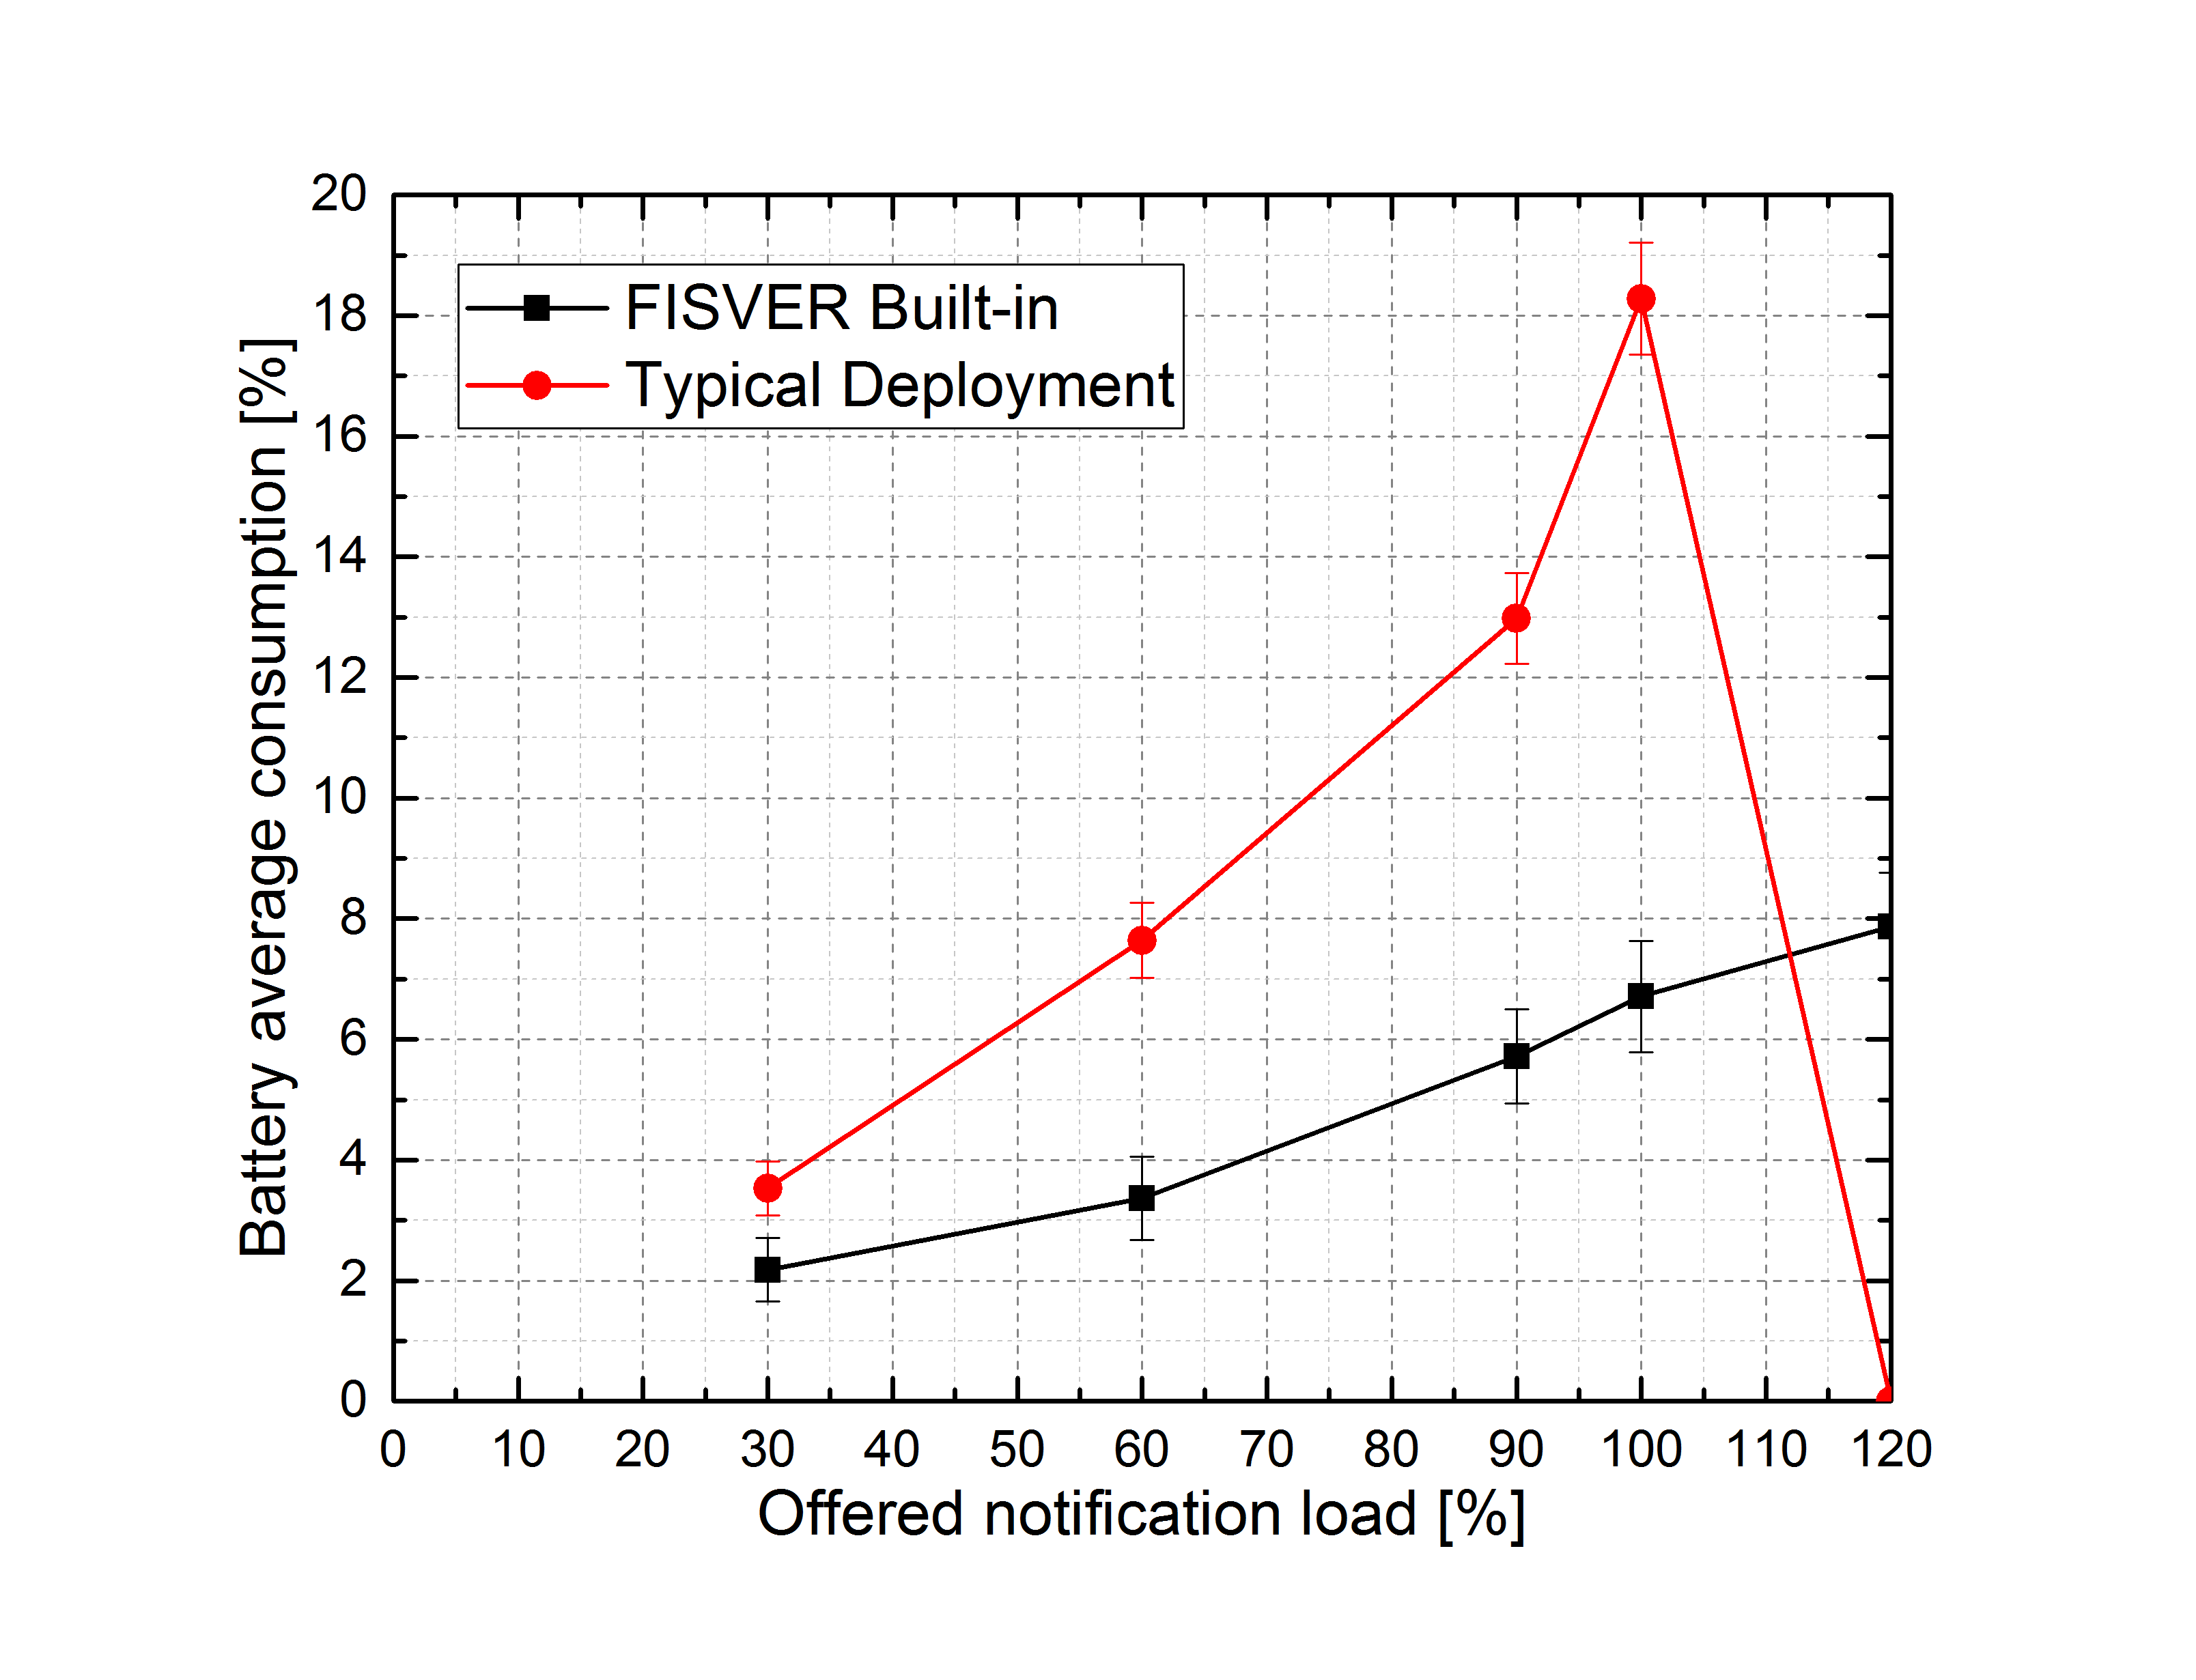
\includegraphics[scale=0.60]{Imagens/cap5_bat.png}
 	\caption{Average battery power consumption in FISVER Built-in and Typical Deployment set of experiments}
 	\label{fig:result1}
\end{figure}

As it can be confirmed from the results scratched by Figure \ref{fig:result1}, the percentage of the energy that is consumed in the Typical Deployment set of experiments follows the same behavior as for both \ref{NetAnalytics} and \ref{CPUAnalytics} in respect to exponential projection with the increasing offered event notification load. This behavior follows the same reasons as for those previous analysis, on the basis that the mobile application side deploys heavyweight processing tasks, whereas a lightweight event-driven approach is provisioned at the FISVER Built-in testbed.

The outcomes analytics expose that FISVER Built-in outperforms the Typical Deployment set of experiments by achieving an average battery consumption performance of 99.54\% (from 4,88\% to 10,61\% respectively). Therefore, this experiment set has proven that streaming-based mobile applications of Typical Deployment scenario is not energy-efficient over the FISVER Built-in approach, by the need for constantly accessing the network and processing video data analytics.

\subsection{Result Analysis Insights}
\label{ResAnalyIns}

The significant improvements in the consumption rates of the battery, CPU and networking resources obtained from the FISVER Built-in set of experiments compared with the Typical Deployment configuration, are essentially explained by the influence of the notification-based cloud approach, which allows a sharp decline in the amount of resource demands at the mobile device.

While the transport safety application generally remains connected in standby mode in the FISVER Built-in set of experiments, the coupled-based approach deployed by the Transport Safety application in the Typical Deployment set of experiments requires frequent data exchanges to gather in-vehicle raw data from the remote system.

The results highlighted in this chapter on the testbed assessments, allow to demonstrate the suitability of FISVER proposal in affording cloud-enabled smart surveillance based transport-safety services, as well as its outstanding performance over the Typical Deployment experiment sets. The FISVER proposal evidences performance improvement in CPU utilization load (75.6\%), upstream(99.993\%)/downstream(99.996\%) throughput and battery consumption (99.54\%) in comparison to the behavior of the Typical Deployment set of experiments.
